\documentclass[11pt,a4paper]{article}
\usepackage[margin=1in]{geometry}
\usepackage[T1]{fontenc}
\usepackage[utf8]{inputenc}
\usepackage{lmodern}
\usepackage{hyperref}
\usepackage{enumitem}
\usepackage{xurl}
\usepackage{tikz}
\usepackage{float}
\usetikzlibrary{arrows.meta, positioning, shapes.geometric}
\hypersetup{colorlinks=true,linkcolor=blue,urlcolor=blue}
\newcommand{\codepath}[1]{\path{#1}}
\tikzset{box/.style={rectangle,draw,rounded corners,align=center,inner sep=3pt,minimum width=36mm},decision/.style={diamond,draw,aspect=2.1,align=center,inner sep=2pt},line/.style={-Latex}}

\title{Phase-1 Deliverable: Residency Model}
\author{SIT Engine Architecture}
\date{\today}

\begin{document}
\maketitle

\section{Technical Description}
The Residency Model provides a canonical representation of residency intervals and residency-conditioned state accounting. Its primary purpose is to guarantee SIT accumulation happens only where residency permits.

\section{Implementation Fulfillment}
Validation contract lives in \codepath{Phase-1/ingest/ingest_api.py} (\texttt{validate\_resid\_df}). Runtime gating is implemented in \codepath{Phase-1/sit_engine_phase1.py} through mask merge/intersection and resident accumulation maps. Invariant enforcement for non-resident behavior is in \codepath{Phase-1/tests/check_invariants.py}.

\section{Design \& Architecture}
Per-core residency intervals are merged into canonical masks. State intervals are clipped against masks before window accumulation. If no residency input exists, full-window residency fallback is used for compatibility.

\subsection*{Function Flowchart}
\begin{figure}[H]
\centering
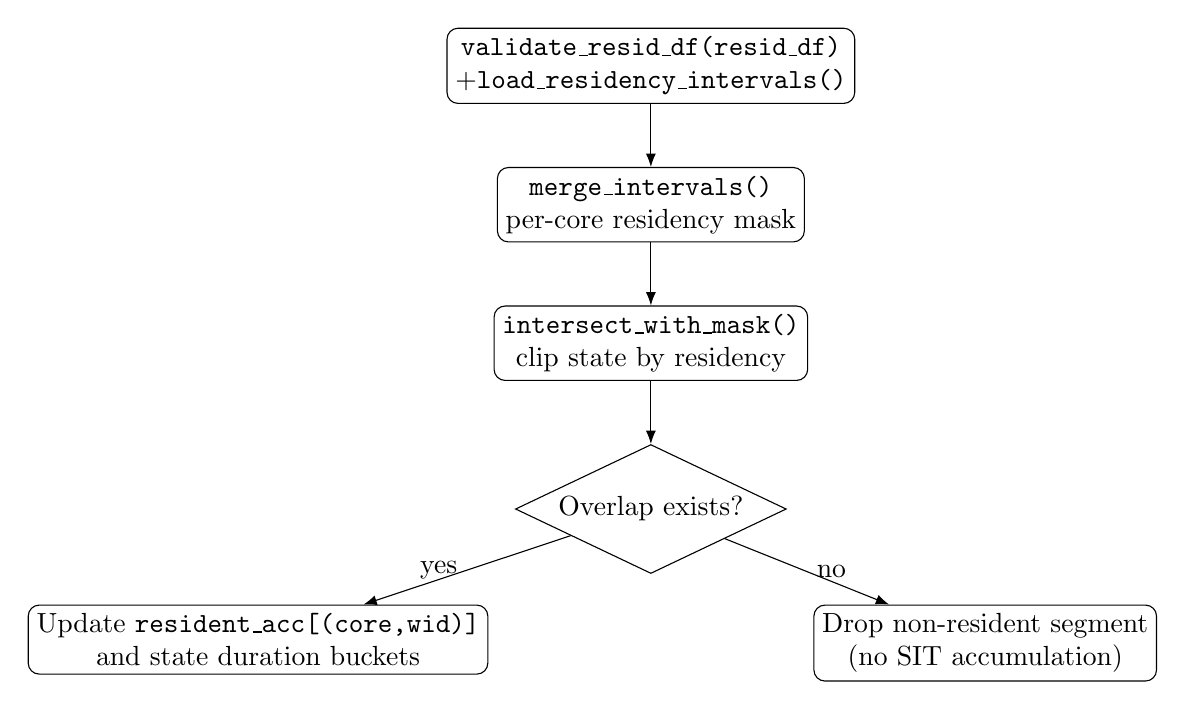
\begin{tikzpicture}[node distance=8mm and 12mm]
\node[box] (a) {\texttt{validate\_resid\_df(resid\_df)}\\+\texttt{load\_residency\_intervals()}};
\node[box, below=of a] (b) {\texttt{merge\_intervals()}\\per-core residency mask};
\node[box, below=of b] (c) {\texttt{intersect\_with\_mask()}\\clip state by residency};
\node[decision, below=of c] (d) {Overlap exists?};
\node[box, below left=of d] (e1) {Update \texttt{resident\_acc[(core,wid)]}\\and state duration buckets};
\node[box, below right=of d] (e2) {Drop non-resident segment\\(no SIT accumulation)};
\draw[line] (a) -- (b);
\draw[line] (b) -- (c);
\draw[line] (c) -- (d);
\draw[line] (d) -- node[left]{yes} (e1);
\draw[line] (d) -- node[right]{no} (e2);
\end{tikzpicture}
\caption{Residency Model Function Flow}
\end{figure}

\end{document}
